\documentclass{beamer}
\usepackage[version=4]{mhchem} 
\usepackage{tikz}


\usetheme{Madrid}
\usecolortheme{beaver}

\title{Unit 3}
\subtitle{Modelado de la estructura atómica}
\author{Mr. Maxwell}
\institute{PACS}
\date{\today}


\begin{document}

\frame{\titlepage}
\frame{\tableofcontents}

\section{Estructura atómica}

%!%%%%%%%% ATOMIC NUMBER  %%%%%%%%%%%%%%%

\subsubsection{Número atómico}

\begin{frame}
    \frametitle{Número atómico}
\onslide The 
 \pause \alert{Número atómico}
 \onslide is the number of 
 \pause \alert{protones} 
 \onslide in the nucleus of an atom.
\end{frame}

%!%%%%%%%% MASS NUMBER  %%%%%%%%%%%%%%%

\subsubsection{Número de masa}
\begin{frame}
    \frametitle{Masa atómica}
    \onslide El
    \pause \alert{número de masa}
    \onslide el número total de
    \pause \alert{protones}
    \onslide y
    \pause \alert{neutrones}
    \onslide en el núcleo de un átomo.
    \end{frame}

%*%%%%%% Hidrógeno %%%%%%%


\begin{frame}
    \frametitle{Hidrógeno}
    $$\ce{^{\alert{1}}_{}H}$$

    \pause ¿Qué significa \alert{1}?\\

    \pause 1 es el número total de neutrones y protones.

    \vspace{1cm}

    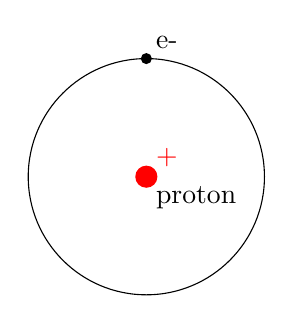
\begin{tikzpicture}
        \coordinate (center) at (0,0);
        \def\radius{1.5cm}
        % a circle
        \draw (center) circle[radius=\radius];
        \fill (center) circle[radius=2pt] node[below right] {proton};
      
        % a random point of the circle
 
        \fill[red] (center) circle[radius=4pt] node[above right] {+};
        \fill[black] (center) ++(90:\radius) circle[radius=2pt]  node[above right] {e-};
    \end{tikzpicture}


\end{frame}


%*%%%%%% Helio %%%%%%%

\begin{frame}
    \frametitle{Helio}
 $$\ce{^{4}_{2}He}$$

 \pause ¿Qué significa \alert{4}?\\
 \pause \alert{4} es el número total de neutrones y protones.\\
 \pause ¿Qué significa \alert{2}?\\
 \pause \alert{2} es el número de protones.

    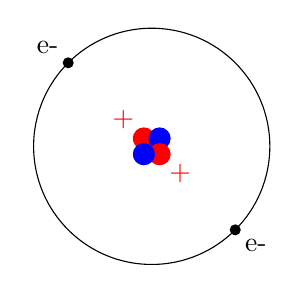
\begin{tikzpicture}

        \coordinate (center) at (0,0);
        \def\radius{1.5cm}
        % a circle
        \draw (center) circle[radius=\radius];

      
        % a random point of the circle
        \fill[red] (-.1, .1) circle[radius=4pt]node[above left] {+};
        \fill[blue] (.1, .1) circle[radius=4pt];
        \fill[red] (.1, -.1) circle[radius=4pt]node[below right] {+};
        \fill[blue] (-.1, -.1) circle[radius=4pt];
        \pause \fill[black] (center) ++(135:\radius) circle[radius=2pt]  node[above left] {e-};
        \pause \fill[black] (center) ++(-45:\radius) circle[radius=2pt] node[below right] {e-};

    \end{tikzpicture}





\end{frame}


%!%%%%%%%%%%% LITHIUM %%%%%%%%%%%%%%

\begin{frame}
    \frametitle{litio}
 $$\ce{^{7}_{3}Li}$$

 \onslide<1->¿Cuántos protones tiene el litio?
 \onslide<2->3
 
 \onslide<3->¿Cuántos neutrones?\\
 \onslide<4-> $7 - 3 = \onslide<5-> 4 $


    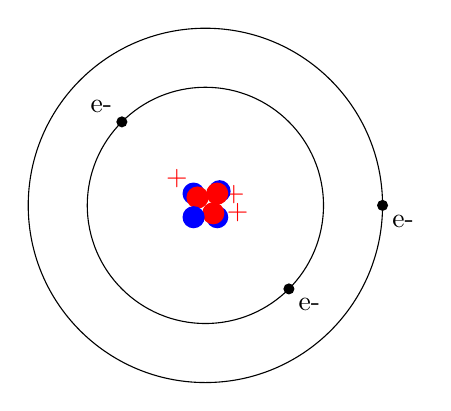
\begin{tikzpicture}

        \coordinate (center) at (0,0);
        \def\radius{1.5cm}
   
        
        \onslide<4->\fill[blue] (-.15, .15) circle[radius=4pt]; 
        \onslide<2->\fill[red] (-.1, .1) circle[radius=4pt]node[above left] {+};  
        \onslide<4->\fill[blue] (.15, -.15) circle[radius=4pt]; 
        \onslide<2->\fill[red] (.1, -.1) circle[radius=4pt]node[above right] {+}; 
        \onslide<4->\fill[blue] (.18, .18) circle[radius=4pt]; 
        \onslide<2->\fill[red] (.15, .15) circle[radius=4pt]node[below right] {+}; 
        \onslide<4->\fill[blue] (-.15, -.15) circle[radius=4pt]; 
        
        
        
        \onslide<6->\draw (center) circle[radius=\radius];
        \onslide<7-> \fill[black] (center) ++(135:\radius) circle[radius=2pt]  node[above left] {e-};
        \onslide<8-> \fill[black] (center) ++(-45:\radius) circle[radius=2pt] node[below right] {e-};
        \onslide<9->\draw (center) circle[radius=\radius*1.5];
        \onslide<10->\fill[black] (center) ++(0:\radius*1.5) circle[radius=2pt] node[below right] {e-};
        
    \end{tikzpicture}

\end{frame}

%*%%%%%%% BOHR %%%%%%%%%%%%%

\subsection{Bohr Model}

\begin{frame}
    \begin{columns}
        \frametitle{Niels Bohr}
        \begin{column}{0.5\textwidth}
            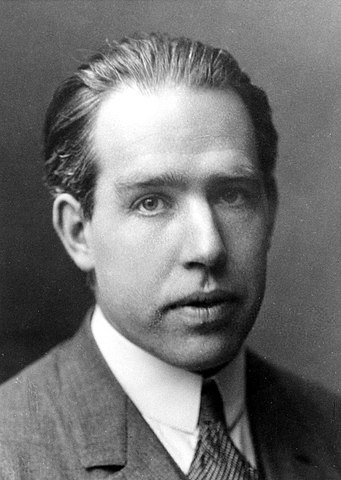
\includegraphics[width=3cm]{../../../../public/images/chemists/Bohr.jpg}
        \end{column}
        \begin{column}{0.5\textwidth}
            El modelo de Bohr: Bohr propuso que un átomo era un núcleo con electrones "orbitando" en diferentes
            \pause \alert{niveles de energía}.
            \vspace{1cm}

        
        \end{column}
    \end{columns}
\end{frame}

%! ENERGY LEVELS %%%%%%%

\subsubsection{Niveles de energía}

\begin{frame}
    \frametitle{Niveles de energía}
    \onslide Los electrones solo pueden tener ciertos valores de energía conocidos como
    \pause \alert{niveles de energía}
\end{frame}

\begin{frame}
    \frametitle{Niveles de energía}
    \onslide Los electrones más cercanos al núcleo tienen la
    \pause \alert{menor}
    \onslide energía, mientras que los que están más lejos tienen la
    \pause\alert{mayor}
    \onslide energía.
    \vspace{.5cm}

    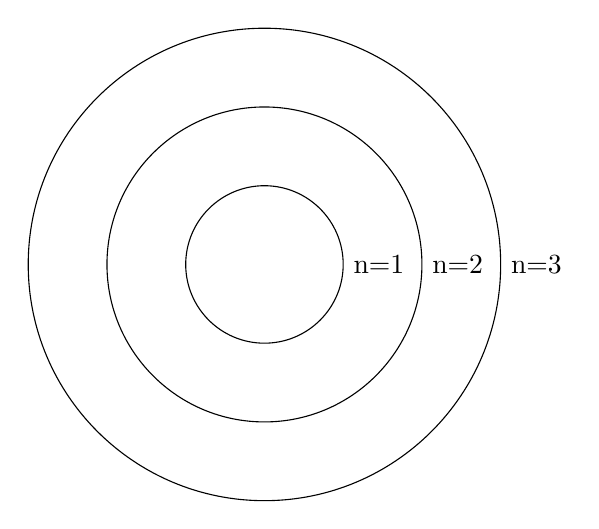
\begin{tikzpicture}
    \foreach \r/\c in {1/n=1, 2/n=2, 3/n=3} 
    {
      \pause \node[circle, draw, minimum size=2*\r cm,label=right:\c] {};
    }
      \end{tikzpicture}
    
\end{frame}



\begin{frame}
    \frametitle{Niveles de energía y la tabla periódica}
    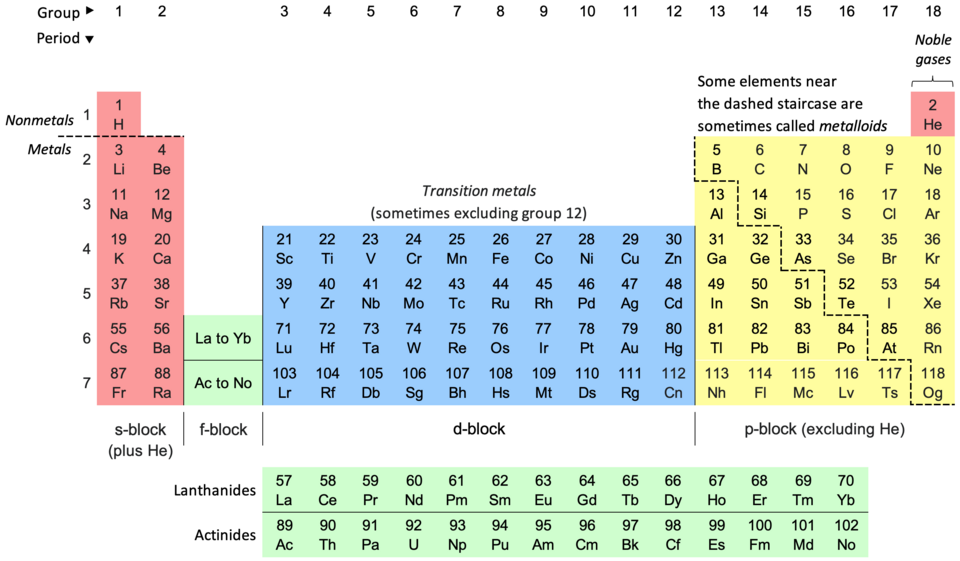
\includegraphics[width=10cm]{../../../../public/images/pTable.png}
\end{frame}

\begin{frame}
    \frametitle{Nivel de energía de Hidrógeno}
    \begin{columns}
        
        \begin{column}{0.5\textwidth}
            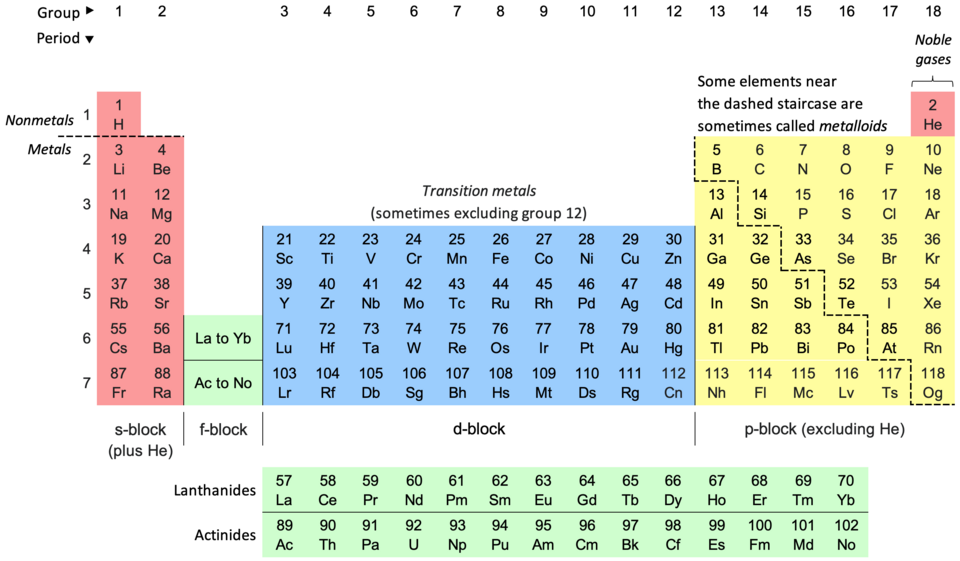
\includegraphics[width=6cm]{../../../../public/images/pTable.png}
            
        \end{column}
        \begin{column}{0.5\textwidth}

            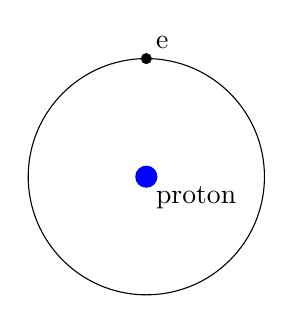
\begin{tikzpicture}
                \coordinate (center) at (0,0);
                \def\radius{1.5cm}
                % a circle
                \draw (center) circle[radius=\radius];
                \fill (center) circle[radius=2pt] node[below right] {proton};
              
                % a random point of the circle
         
                \fill[blue] (center) circle[radius=4pt];
                \fill[black] (center) ++(90:\radius) circle[radius=2pt]  node[above right] {e};
            \end{tikzpicture}
            
        \end{column}
    \end{columns}

\end{frame}

\begin{frame}
    \frametitle{Nivel de energía de litio}
    \begin{columns}
        
        \begin{column}{0.5\textwidth}
            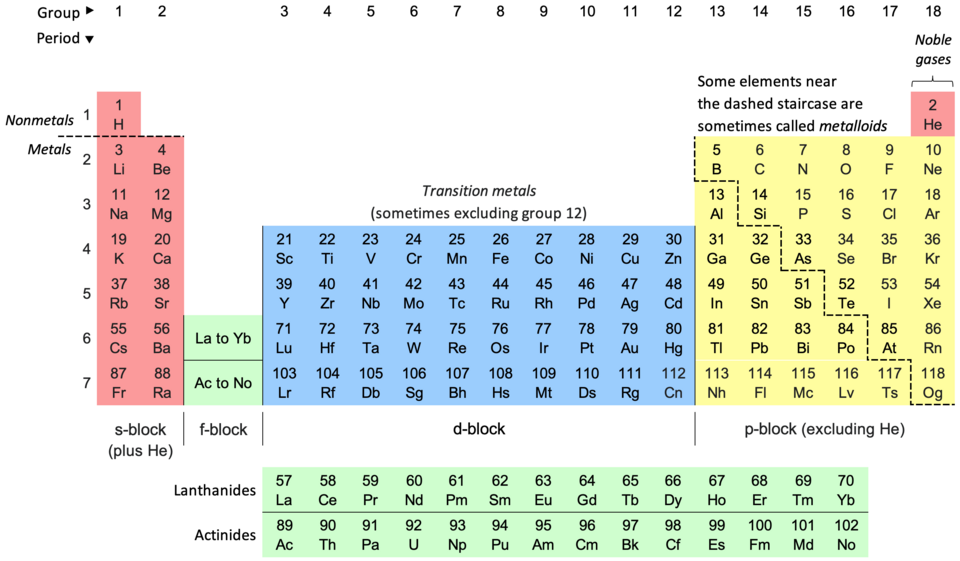
\includegraphics[width=6cm]{../../../../public/images/pTable.png}
            
        \end{column}
        \begin{column}{0.5\textwidth}
            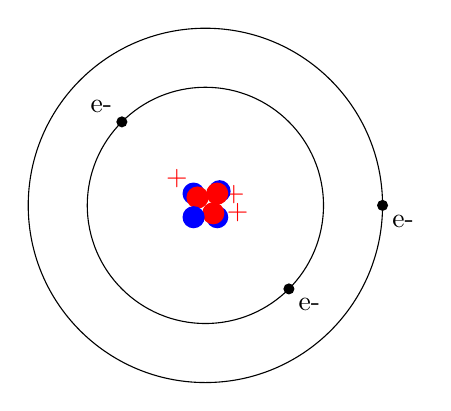
\begin{tikzpicture}
                \coordinate (center) at (0,0);
                \def\radius{1.5cm}
           
                
                \onslide<4->\fill[blue] (-.15, .15) circle[radius=4pt]; 
                \onslide<2->\fill[red] (-.1, .1) circle[radius=4pt]node[above left] {+};  
                \onslide<4->\fill[blue] (.15, -.15) circle[radius=4pt]; 
                \onslide<2->\fill[red] (.1, -.1) circle[radius=4pt]node[above right] {+}; 
                \onslide<4->\fill[blue] (.18, .18) circle[radius=4pt]; 
                \onslide<2->\fill[red] (.15, .15) circle[radius=4pt]node[below right] {+}; 
                \onslide<4->\fill[blue] (-.15, -.15) circle[radius=4pt]; 
                
                
                
                \onslide<6->\draw (center) circle[radius=\radius];
                \onslide<7-> \fill[black] (center) ++(135:\radius) circle[radius=2pt]  node[above left] {e-};
                \onslide<8-> \fill[black] (center) ++(-45:\radius) circle[radius=2pt] node[below right] {e-};
                \onslide<9->\draw (center) circle[radius=\radius*1.5];
                \onslide<10->\fill[black] (center) ++(0:\radius*1.5) circle[radius=2pt] node[below right] {e-};
                
            \end{tikzpicture}
            
        \end{column}
    \end{columns}

\end{frame}

\begin{frame}
    \frametitle{Nivel de energía de Sodium}
    \begin{columns}
        
        \begin{column}{0.5\textwidth}
            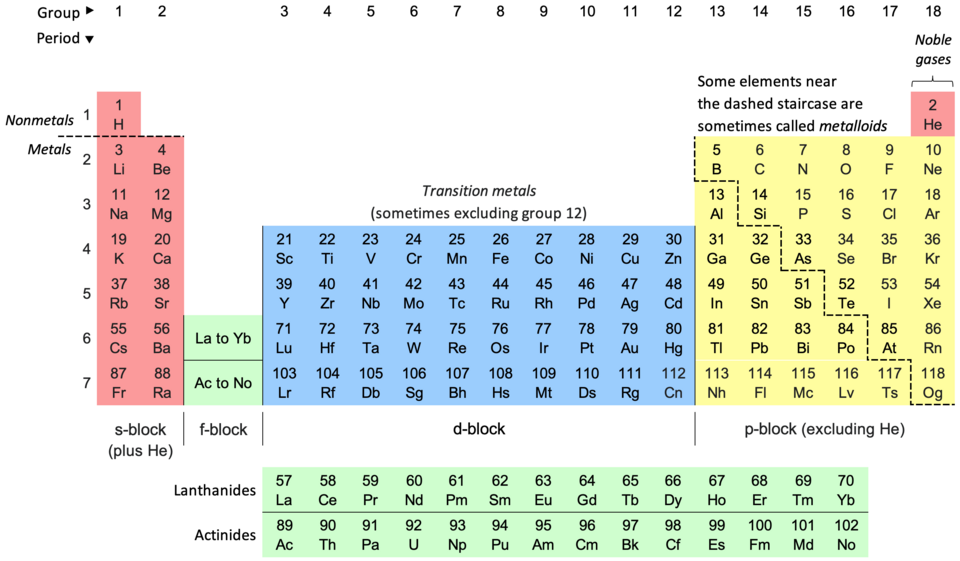
\includegraphics[width=6cm]{../../../../public/images/pTable.png}
            
        \end{column}
        \begin{column}{0.5\textwidth}
            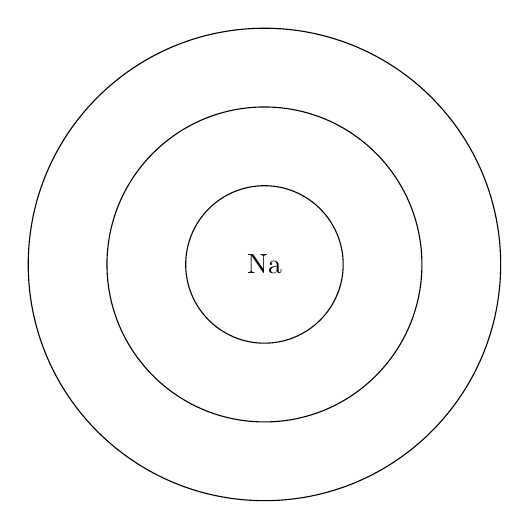
\begin{tikzpicture}
                \foreach \r/\c in {1/Na, 2/, 3/} { \pause \node[circle, draw, minimum size=2*\r cm,label=center:\c] {};}
                \end{tikzpicture}
            
        \end{column}
    \end{columns}

\end{frame}

%%%%%! PERIODIC TABLE %%%%%%%


\subsection{La tabla periódica}

\subsubsection{grupos y periodos}

\begin{frame}
    \frametitle{La tabla periódica}

    \onslide La tabla periódica has
    \pause \alert{7}
    \onslide períodos y
    \pause \alert{18}
    \onslide grupos.
    
    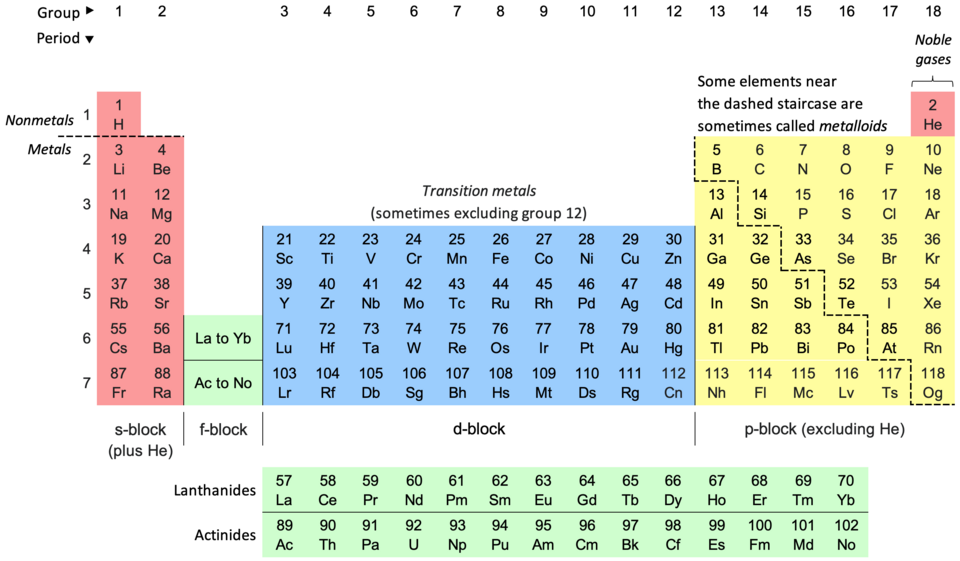
\includegraphics[width=10cm]{../../../../public/images/pTable.png}

\end{frame}


\begin{frame}
    \frametitle{Horizontal and Vertical}
    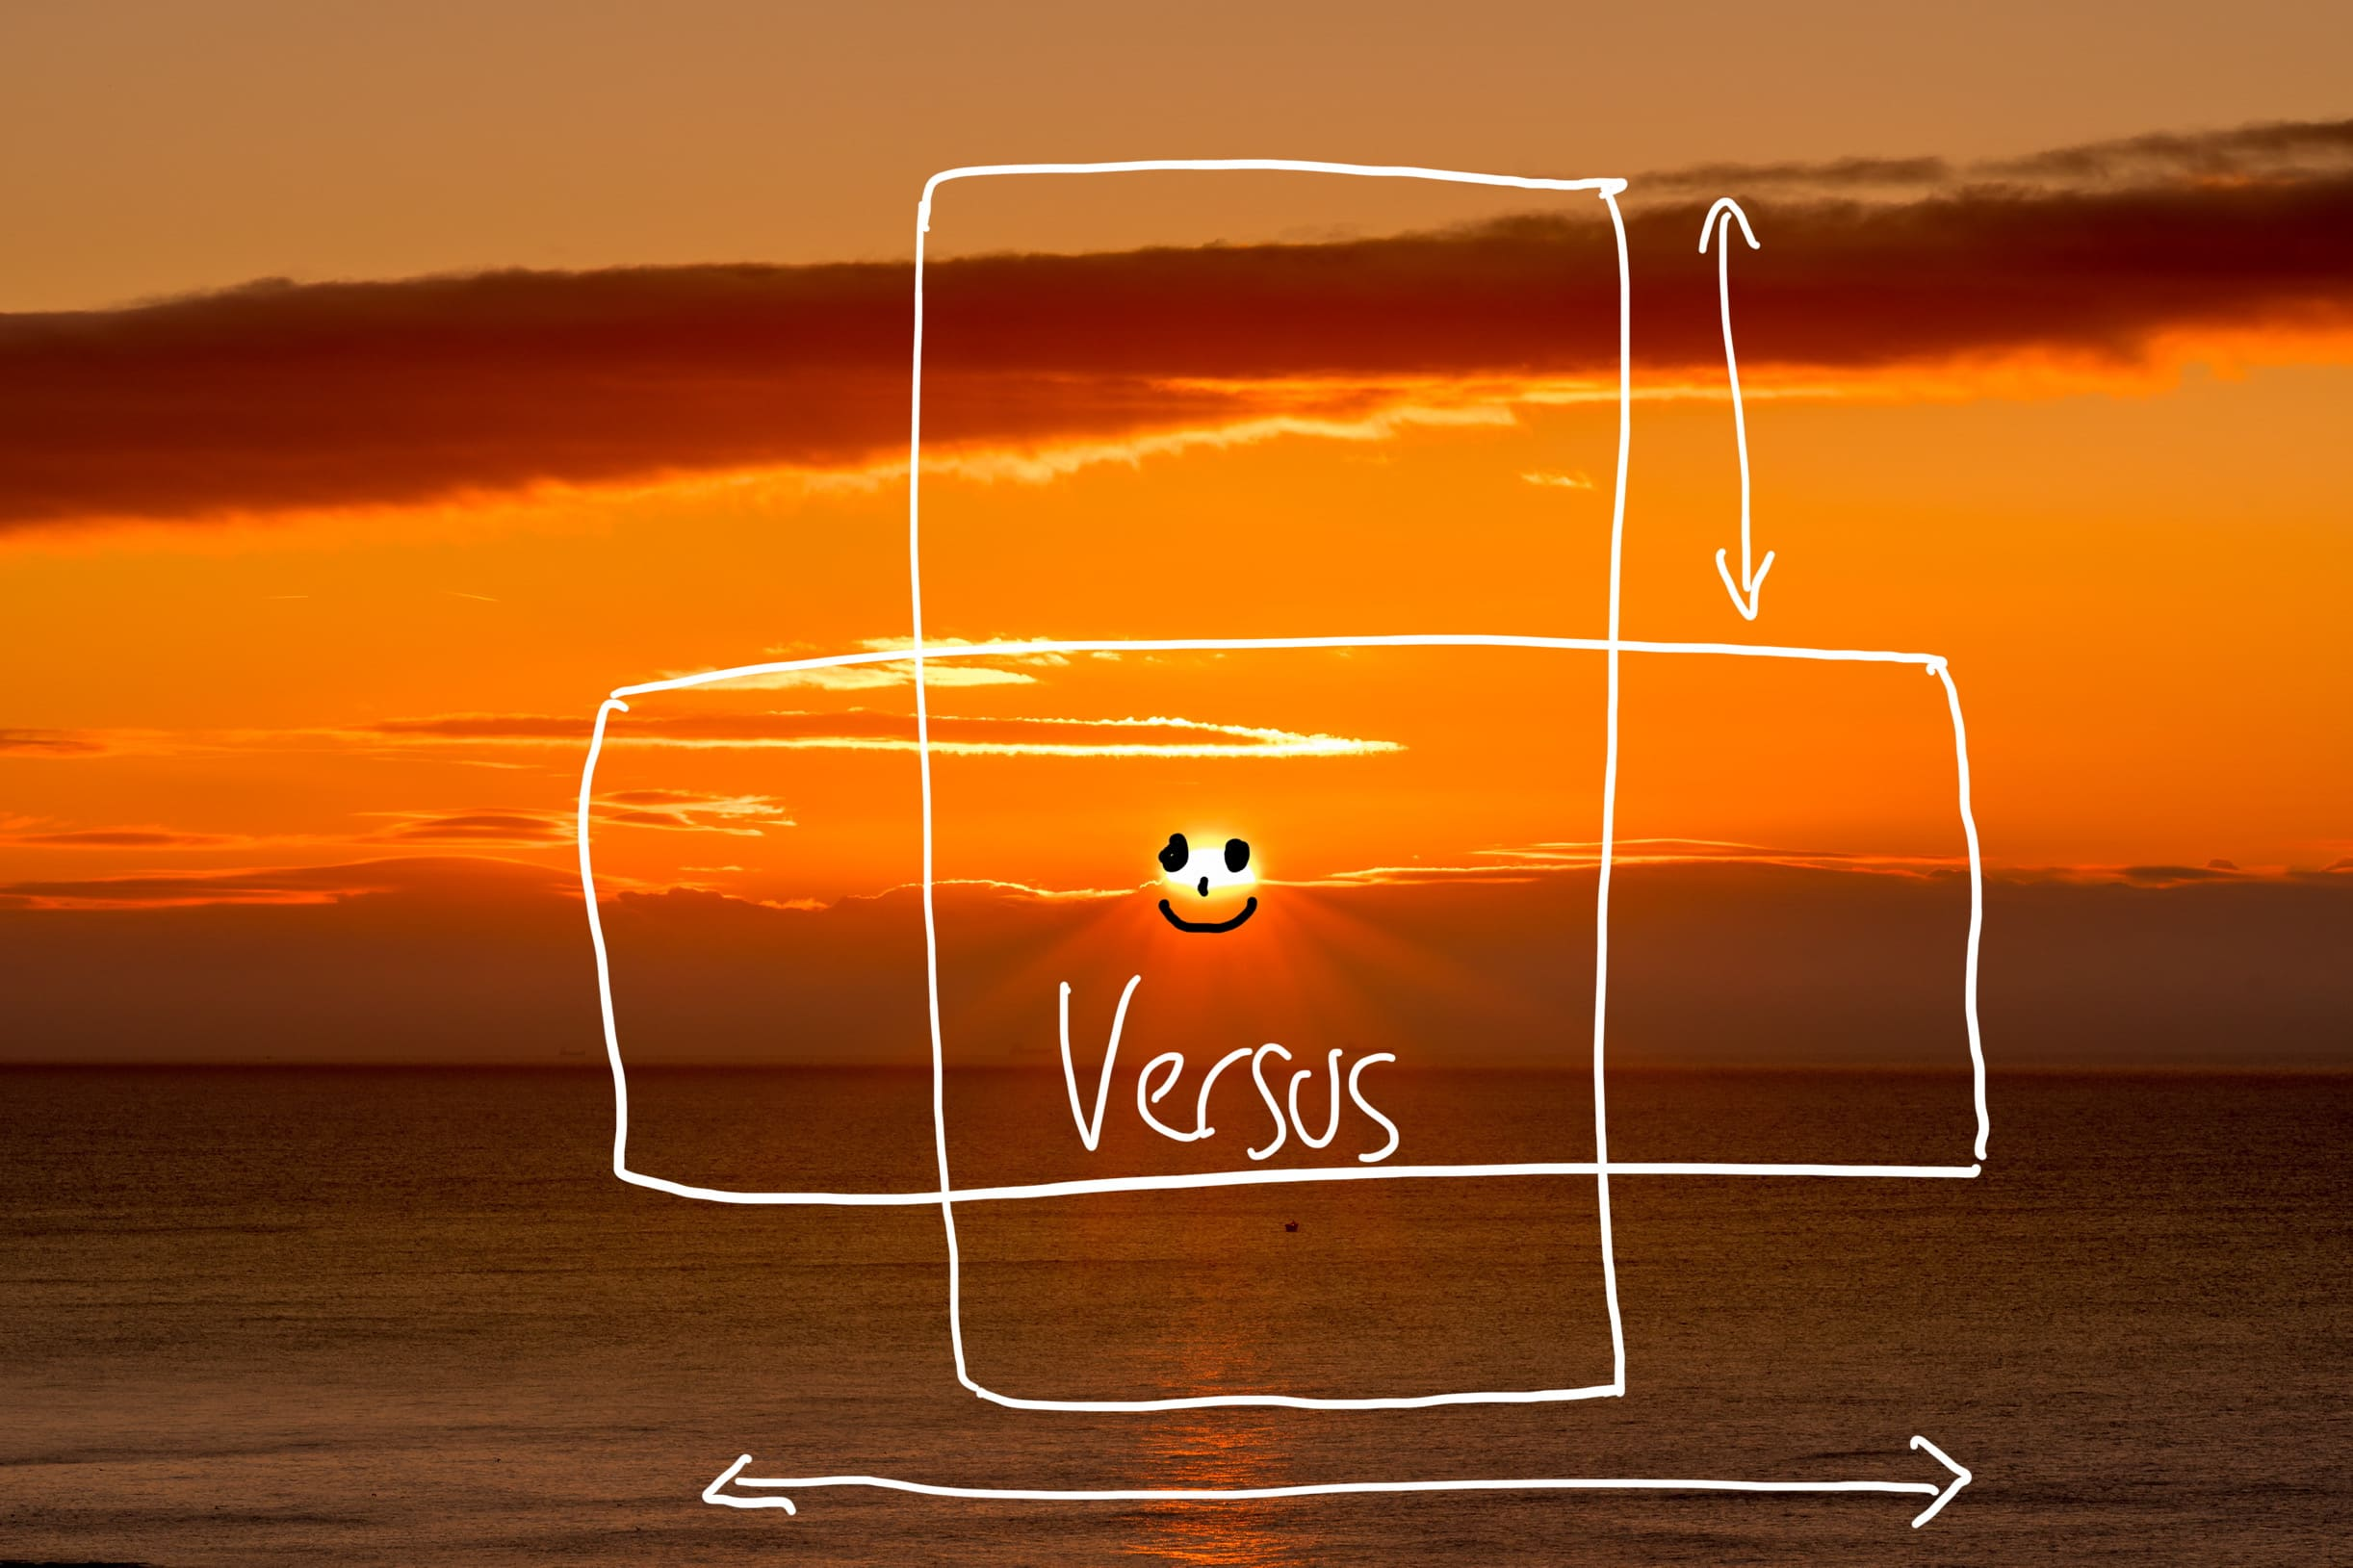
\includegraphics[width=10cm]{../../../../public/images/hor_vert.jpg}

    \onslide Los períodos son
    \pause \alert{horizontales}
    \onslide y los grupos son
    \pause \alert{verticales}.
\end{frame}

\begin{frame}


\frametitle{Nivel de energía de Hidrógeno}
        \begin{columns}
            %%%%%%%%? FIRST COLUMN %%%%%
            \begin{column}{0.5\textwidth}
                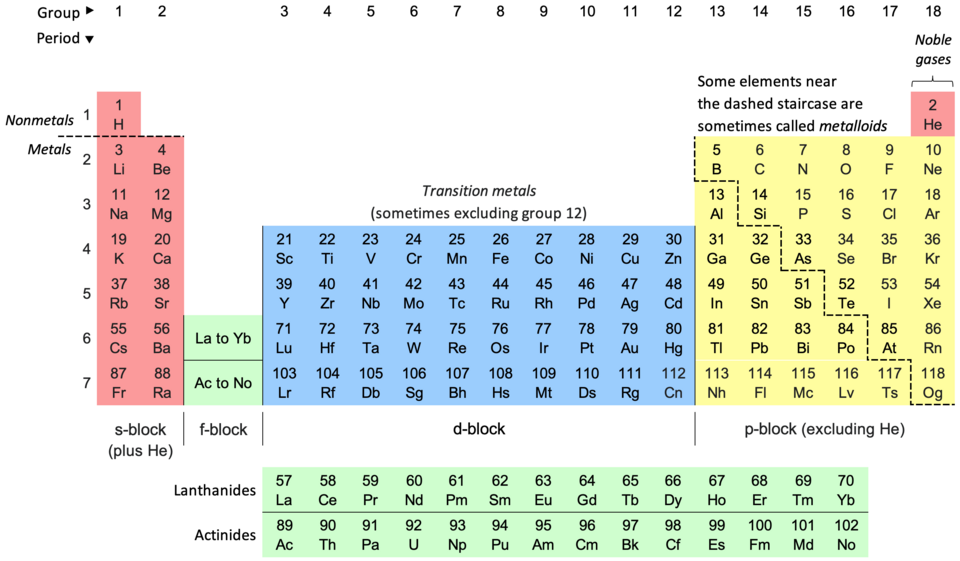
\includegraphics[width=6cm]{../../../../public/images/pTable.png}
                
            \end{column}

            %%%%%%%%? SECOND COLUMN %%%%%
            \begin{column}{0.5\textwidth}
    
                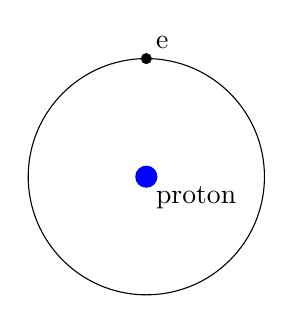
\begin{tikzpicture}
                    \coordinate (center) at (0,0);
                    \def\radius{1.5cm}
                    % a circle
                    \draw (center) circle[radius=\radius];
                    \fill (center) circle[radius=2pt] node[below right] {proton};
                  
                    % a random point of the circle
             
                    \fill[blue] (center) circle[radius=4pt];
                    \fill[black] (center) ++(90:\radius) circle[radius=2pt]  node[above right] {e};
                \end{tikzpicture} 
            \end{column}
        \end{columns}
    
        \vspace{1cm}

        \onslide Puedes conocer la configuración
        \pause \alert{electrón}
        \onslide de un elemento a partir de su
        \pause \alert{posición}
    \onslide in La tabla periódica. 
\end{frame}



\begin{frame}


    \frametitle{Nivel de energía de Hidrógeno}
    \begin{columns}
        
        \begin{column}{0.5\textwidth}
            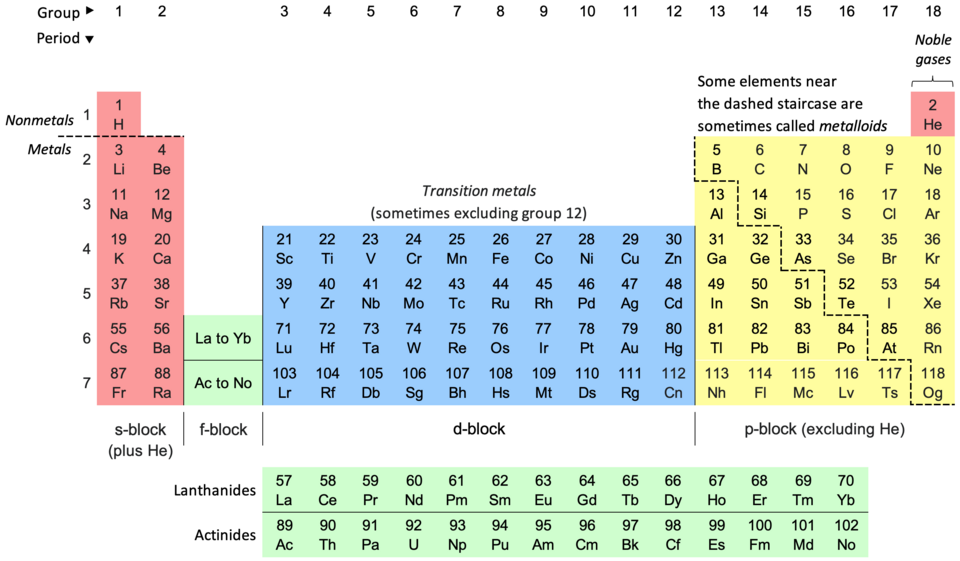
\includegraphics[width=6cm]{../../../../public/images/pTable.png}
            
        \end{column}
        \begin{column}{0.5\textwidth}

            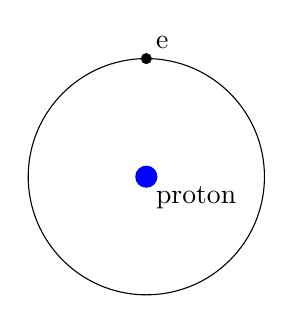
\begin{tikzpicture}
                \coordinate (center) at (0,0);
                \def\radius{1.5cm}
                % a circle
                \draw (center) circle[radius=\radius];
                \fill (center) circle[radius=2pt] node[below right] {proton};
              
                % a random point of the circle
         
                \fill[blue] (center) circle[radius=4pt];
                \fill[black] (center) ++(90:\radius) circle[radius=2pt]  node[above right] {e};
            \end{tikzpicture}
            
        \end{column}
    \end{columns}

    \vspace{1cm}

    \onslide El número de capas de electrones
    \pause \alert{}
    \onslide (o niveles de energía) es igual al número
    \pause \alert{período}
    \onslide .


\end{frame}


%%%%%%%%%! Electrones de valencia %%%%%%%%

\subsection{Electrones de valencia}


\begin{frame}


    \frametitle{Electrones de valencia}
    \begin{columns}
        
        \begin{column}{0.5\textwidth}
            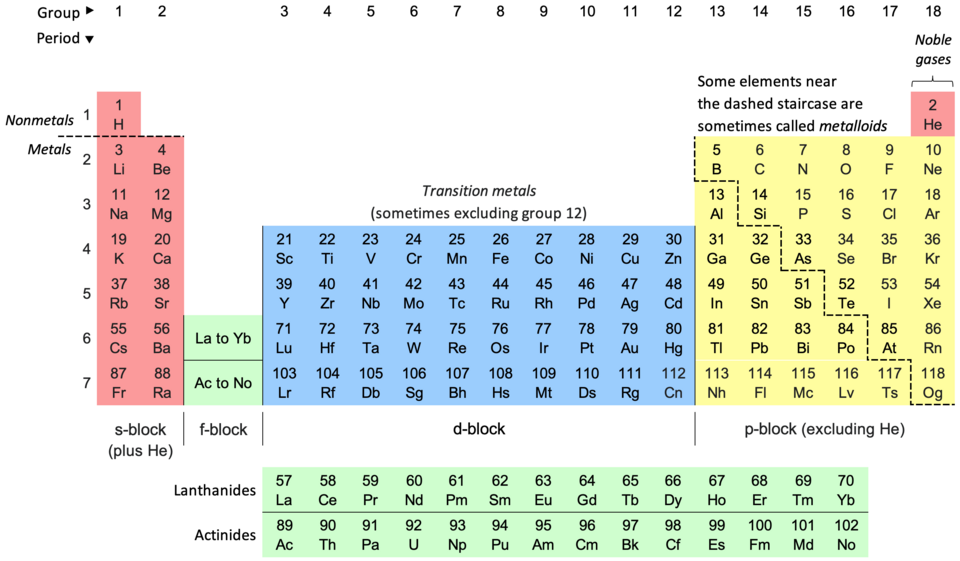
\includegraphics[width=6cm]{../../../../public/images/pTable.png}
            
        \end{column}
        \begin{column}{0.5\textwidth}

            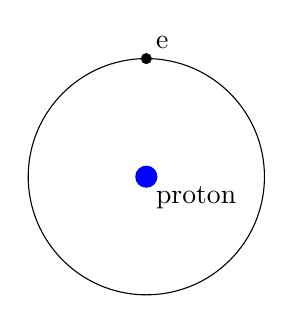
\begin{tikzpicture}
                \coordinate (center) at (0,0);
                \def\radius{1.5cm}
                % a circle
                \draw (center) circle[radius=\radius];
                \fill (center) circle[radius=2pt] node[below right] {proton};
              
                % a random point of the circle
         
                \fill[blue] (center) circle[radius=4pt];
                \fill[black] (center) ++(90:\radius) circle[radius=2pt]  node[above right] {e};
            \end{tikzpicture}
            
        \end{column}
    \end{columns}

    \vspace{1cm}

    \onslide El número de electrones de valencia está relacionado con el número de
    \pause \alert{grupo}.


\end{frame}


\begin{frame}


    \frametitle{Electrones de valencia}
    \begin{columns}
        
        \begin{column}{0.5\textwidth}
            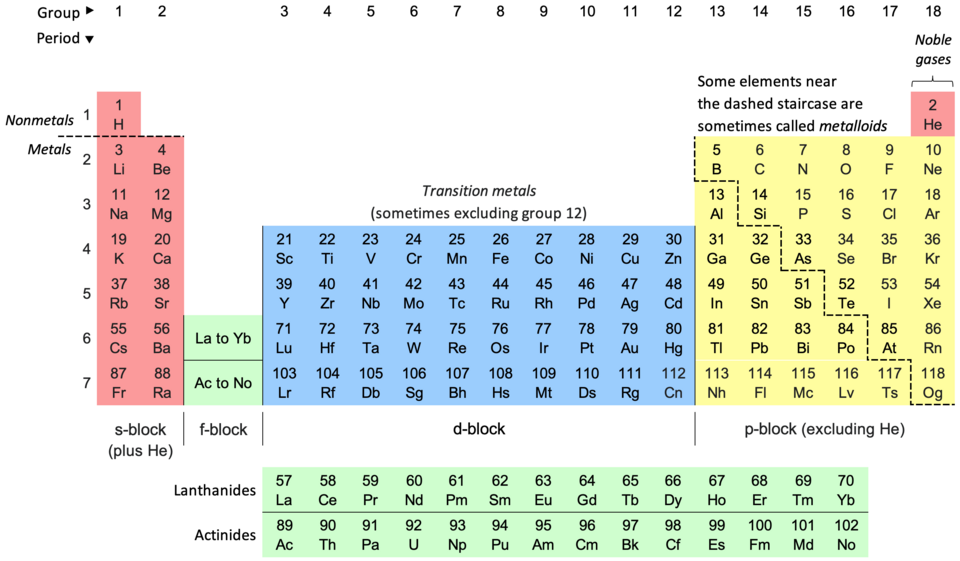
\includegraphics[width=6cm]{../../../../public/images/pTable.png}
            
        \end{column}
        \begin{column}{0.5\textwidth}

            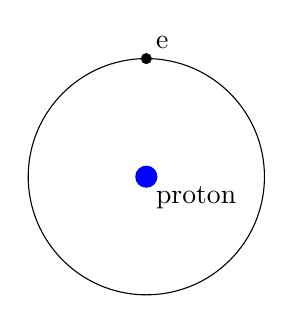
\begin{tikzpicture}
                \coordinate (center) at (0,0);
                \def\radius{1.5cm}
                % a circle
                \draw (center) circle[radius=\radius];
                \fill (center) circle[radius=2pt] node[below right] {proton};
              
                % a random point of the circle
         
                \fill[blue] (center) circle[radius=4pt];
                \fill[black] (center) ++(90:\radius) circle[radius=2pt]  node[above right] {e};
            \end{tikzpicture}
            
        \end{column}
    \end{columns}

    \vspace{1cm}

    \onslide Para los átomos en los grupos
    \pause \alert{uno}
    \onslide y
    \pause \alert{dos},
    \onslide el número de
    \pause \alert{electrones de valencia}
    \onslide son iguales al número del grupo.
    
    \vspace{1cm}
    

    \onslide Para los átomos de los grupos
    \pause \alert{13}
    \onslide a
    \pause \alert{18},
    \onslide el número de
    \pause \alert{electrones de valencia}
    \onslide son iguales al número del grupo menos 10.
\end{frame}

%! EXAMPLES

\begin{frame}
    \frametitle{Electrones de valencia of \ce{Li}}
    \begin{columns}
        
        \begin{column}{0.5\textwidth}
            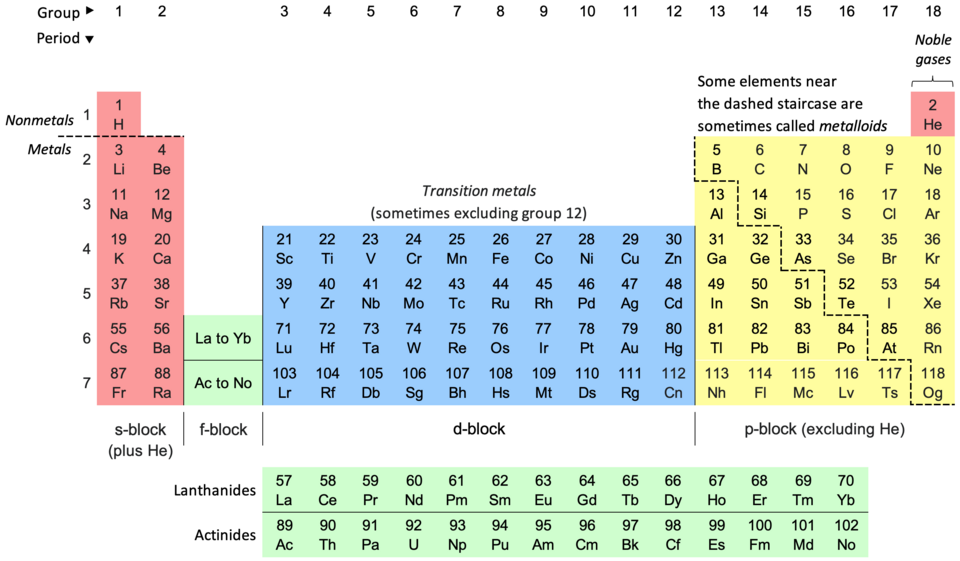
\includegraphics[width=6cm]{../../../../public/images/pTable.png}
            
        \end{column}
        \begin{column}{0.5\textwidth}

            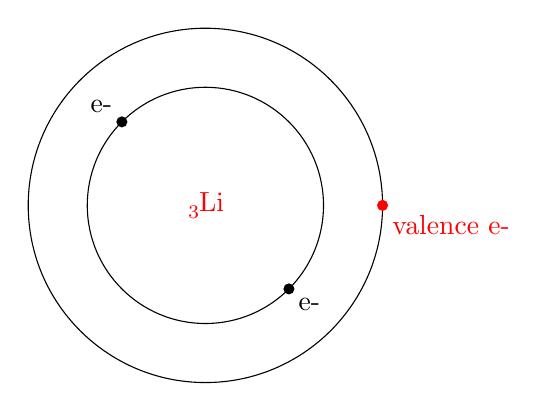
\begin{tikzpicture}

                \coordinate (center) at (0,0);
                \def\radius{1.5cm}
           
                
                \fill[red] (center) node {$$\ce{^{}_{3}Li}$$}; 
                
                
                
                \draw (center) circle[radius=\radius];
                 \fill[black] (center) ++(135:\radius) circle[radius=2pt]  node[above left] {e-};
                 \fill[black] (center) ++(-45:\radius) circle[radius=2pt] node[below right] {e-};
                \draw (center) circle[radius=\radius*1.5];
                \onslide<2->\fill[red] (center) ++(0:\radius*1.5) circle[radius=2pt] node[below right] {valence e-};
                
            \end{tikzpicture}
            
        \end{column}
    \end{columns}

\end{frame}



\end{document}